\documentclass[../report.tex]{subfiles}
\begin{document}
	
	
	\chapter*{Введение}
	\addcontentsline{toc}{chapter}{Введение}
	\markboth{Введение}{Введение}
	В работе представляются результаты, полученные автором при решении задач, связанных с построением и применением моделей с марковскими переключениями состояний из семейства MS-VARX и сезонной ARIMA-модели (SARIMAX), использующих индекс экономических настроений и индексы доверия белорусской экономики на основе опросных данных системы мониторинга Национального банка Республики Беларусь.
	
	Исследования в данном направлении проводились в Белорусском государственном университете в 2016-2017 гг. в рамках НИР "Разработка системы опережающих экономических индикаторов и экономических диффузных индексов для основных видов экономической деятельности и экономики Республики Беларусь в целом с использованием экономико-математических, эконометрических методов и моделей на основе данных системы мониторинга предприятий Национального банка Республики Беларусь".
	
	Модельный и программный инструментарий для построения указанных  индексов и их применения в предиктивных эконометрических моделях для реального ВВП, а также в моделях с марковскими переключениями состояний для анализа бизнес-цикла белорусской экономики представлены в заключительном отчете о НИР \cite{esiMaking}.
	
	
	
	\chapter{Проблема анализа экономических циклов и основные подходы к ее решению}
	
	\section{Понятие экономического цикла и его интерпретация}
	
	\iffalse
	
	Экономический цикл (бизнес–цикл), согласно определению У–К. Митчелла \cite{mitchellBS}, можно интерпретировать как тип колебаний в общей деловой активности, которая состоит из экспансий, происходящих примерно одновременно в различных видах деятельности, следующих за ними и сопоставимыми по распространенности замедлениями, спадами, оживлениями; ... [без] четкой периодичности; ... [могут] длиться от одного года до десяти или двенадцати лет; бизнес–циклы не могут быть подразделены на более короткие циклы со схожими характеристиками и амплитудой.»  В данной работе рассматриваются преимущественно краткосрочные циклы, с периодом в порядке 2–3 года (циклы Китчена).
	
	NBER США разбивает циклы на фазы сокращения и экспансии. Рассматривается повышение/понижение активности относительно «нормального» уровня. Общая экономическая активность сама характеризуется не только отдельной цифрой ВВП, но и доходами, занятостью, уровнем активности отдельных отраслей \cite{nberDevelopment}. Из–за стабилизации долгосрочных темпов роста экономик к концу ХХ в. изменилась методолония – начали рассматриваться темпы роста экономики (ускорение или замедление относительно долговременного тренда), а также подразделение цикла на 4 части: экспансия (рост над долгосрочным трендом), замедление (падение над трендом), сжатие (снижение под трендом), и восстановление (рост под трендом) \cite{oecdCLI}.
	\fi
	
	\iffalse
	Unused material
	
	Предполагается, что поворотные точки опережающих индикаторов предшествуют поворотным точкам некоторого базового экономического индикатора (например, реального ВВП), характеризующего состояние экономики в целом. В настоящее время существуют два основных методологических центра по разработке подобных индикаторов:   Национальное бюро экономических исследований (НБЭИ) США  (National Bureau of Economic Research – NBER) и Статистический  департамент Организации экономического сотрудничества и развития (ОЭСР) (Organization for Economic Cooperation and Development – OECD). 
	\fi
	
	В рамках концепции экономического цикла, используемой в НБЭИ (Национальное бюро экономических исследований) США, подразумевается последовательная смена двух фаз базового экономического индикатора, называемых периодами «роста» (growth)  и «спада» (recessions) экономической активности. При этом поворотные точки соответствуют «пику» (максимальной точке роста) и «дну» (минимальной точке спада) экономического цикла \cite{nberDevelopment}.  В рамках концепции ОЭСР (Организации экономического сотрудничества и развития) допускается  детализация основных фаз цикла относительно долгосрочного тренда с выделением периодов «роста» и «замедления» (выше линии тренда), а также  – «спада» и «восстановления»  (ниже линии тренда) \cite{oecdCycleExtraction}. Поворотные точки в данном случае соответствуют моментам начала замедления роста и начала восстановления после спада. 
	
	Одной из ключевых задач анализа и прогнозирования экономической активности является разработка систем раннего обнаружения смены фаз экономических циклов на основе специально разработанных экономических индикаторов. Для получения ранних сигналов о смене фаз и оценивания моментов смены фаз, называемых поворотными точками, в рамках указанных систем применяются так называемые опережающие экономические индикаторы (leading economic indicators) \cite{oecdCLI}. В рамках \cite{esiMaking,esiExtra} была разработана система опережающих индикаторов для Республики Беларусь, в том числе Индекс Экономических Настроений/Economic Sentiment Indicator (ИЭН/ESI). В настоящей работе в качестве опережающего и базового экономических индикаторов используются соответственно временные ряды значений индекса экономических настроений, а также реального ВВП Республики Беларусь в ценах 2014 г. в месячном исчислении с мая 2005 г. по январь 2017 г., полученные в рамках указанной НИР.
	
	
	\section{Методы выделения циклической составляющей}
	
	Для периодизации экономических циклов необходимо выделить из временных рядов реального ВВП и ИЭН циклические составляющие, на основании которых затем оцениваются поворотные точки циклов. На опережающий характер ИЭН указывает тот факт, что поворотные точки его цикла предшествуют поворотным точкам цикла реального ВВП. В настоящее время, основным методом выделения догосрочной циклической состовляющей являются статистические фильтры. Наиболее популярным является фильтр Ходрика – Прескотта \cite{oecdCycleExtraction,estrellaFilterDo}. Данный фильтр используется в указанной выше НИР, а так же в рамках данной работы. 
	
	В недавней статье Дж. Хамильтона \cite{hamHP} указывается на проблемы, возникающие при использовании фильтра Ходрика – Прескотта, и предлагается свой метод выделения долгосрочного цикла. Этот метод, так называемый "фильтр Хамильтона", также подвергается некоторой критике.
	
	В проводимом исследовании используются оба метода, т.е. метод Ходрика – Прескотта и метод Хамильтона для выделения долгосрочного цикла, и проводится сравнительный анализ поворотных точек циклов, получаемых с помощью данных фильтров, а так же экспертным путем. Подобное исследование ранее не проводилось на белорусских данных \cite{makarevich_bsu_conf_2017}.
	
	
	\section{Методы оценивания поворотных точек}
	
	Для оценки поворотных точек существуют несколько широко используемых методов. Один из самых популярных – алгоритм Брай – Бошана \cite{bryCyclicalAnalysis}, который состоит из несколько этапов (с минимальной длительностью цикла в 15 месяцев и отдельных фаз в 5 месяцев). Другой популярный метод – модели с переключающимися режимами, впервые популяризированый работой Хамильтона \cite{hamNewApproach}. Результаты Хамильтона с MS-AR для бизнес–цикла США во многом сходились с периодизацией NBER. Многие научные исследования \cite{bodmanCanada,brunoItaly,hardingTwoMethods} указывают на сопоставимость Марковских моделей и традиционных методов, однако на практике они редко используется из–за сравнительной трудоемкости и непрозрачности. Существуют и другие подходы, которые так же не используются из–за сравнительной сложности вычислений.
	
	В данной работе используюся оба подхода для решения указанной задачи.
	
	
	
	\chapter{Эконометрические модели и методы анализа циклических изменений в экономике}
	
	
	\section{Методы выделения и сравнительного анализа экономических циклов}
	
	\subsection{Метод выделения циклов, основанный на фильтре Ходрика – Прескотта}
	
	Приведем краткое описание метода выделения цикла на основе двойного применения фильтра Ходрика – Прескотта. Смысл фильтрации – выделение колебаний в разных частотных диапазонах. Временной ряд рассматривается в представлении $ x_{t} = \tau_{t} + c_{t} + \epsilon_{t}$, где временные ряды $\tau_{t}$ и $c_{t}$, $\epsilon_{t}$ соответствуют трендовой, циклической и случайной шумовой компонентам. Для выделения тренда $\tau_{t}$ решается оптимизационная задача:
	
	\begin{equation} 
	f(\tau, \lambda) = \sum_{t=1}^{T} (y_t-\tau_{t})^2 + \lambda \sum_{t=2}^{T-1} (\tau_{t+1} - 2\tau_{t} + \tau_{t-1}) \rightarrow \min_{\tau} 
	\end{equation}
	
	по значениям $\tau_{t}$, где $\lambda > 0$ – параметр сглаживания тренда: при $\lambda \rightarrow 0$  значения тренда близки к значениям исходного ряда, т. е.  $\tau_{t} \rightarrow y_{t}$, а при $\lambda \rightarrow \infty$ вид тренда приближается  к линейной по времени $t$  функции.
	
	Согласно методике рассмотренной в \cite{esiMaking,esiExtra}, эмпирическим путем были получены значения $\lambda$ соответствующие выделению трендовой составляющей ($\lambda=42131.155$ для циклов длиной 90 месяцев) и сглаживанию циклической состовляющей ($\lambda=13.93$ для циклов длиной 12 месяцев). Если сравнить с методологией ОЭСР \cite{oecdCycleExtraction}, то отличается значение первого параметра из–за различной продолжительности долговременных циклов ($\lambda=133107.94$ для циклов длиной 120 месяцев).
	
	Полная процедура выделения циклов состоит из нескольких этапов. Производится нормализация ряда, затем происходит сезонная корректировка с X13-ARIMA-SEATS \cite{seasonalManual}, выделяется и исключается долговременный тренд первым фильтром, а потом выделяется и сохраняется циклическая составляющая вторым фильтром (для сглаживания/удаления шума). Далее идет оценка поворотных точек (в методологии ОЭСР \cite{oecdCycleExtraction} используется алгоритм Брай–Бошана).
	
	\subsection{Метод сезонной корректировки и выделения циклов, основанной на фильтре Хамильтона}
	
	Сравнительно новый метод выделения циклов был предложен Хамильтоном \cite{hamNewApproach}. В так называемом <<фильтре Хамильтона>>, долгосрочный тренд в нестационарном временном ряду $y_t$  описывается моделью регрессии, включающей, для момента времени  $t+h \quad (h>0)$, константу и $d$ наиболее близких к моменту времени $t$ значения временного ряда:
	
	\begin{equation}
	y_{t+h} = \hat{\alpha_{0}} + \hat{\alpha_{1}}y_{t} + \hat{\alpha_{2}}y_{t-1}
	+ ... + \hat{\alpha_{d}}y_{t-d+1} + \hat{\eta_{t}}
	\end{equation}
	
	где $h$ – априорно задаваемый параметр, зависящий от предполагаемой длины цикла, а остатки модели $\hat{\eta_{t}}$ – исходный ряд с убранным трендом. В статье предлагается брать $d=4$; такое значение $d$ было взято и для описанной в данной работе имплементации в R и Python \cite{makarevich_bsu_conf_2017}. Хамильтоном показано, что при таком выборе параметров для нестационарных интегрированных временных рядов вплоть до порядка $d=4$ остаточная циклическая составляющая $\eta_{t}$ временного ряда вида включает как циклическую, так и стационарную случайную компоненту. 
	
	
	\subsection{Анализ поворотных точек экономических циклов на основе экономических индикаторов}
	
	Для анализа циклов также можно использовать модели, основанные на экономических индикаторах (Economic Indicator Analysis – EIA), в том числе опережающих индикаторов (Compound/Composite Leading Indicator – CLI). Построение таких новых индикаторов на основе уже существующих описано в методологии ОЭСР \cite{oecdCLI} для их исследований. 
	
	Методология ОЭСР использовалась для построения Индекса Экономических Настроений в рамках НИР \cite{esiMaking}. В рамках этой НИР было разработано программное обеспечение на языке R \textbf{ESIanalysis}, а также модельный инструментарий, включающий предиктивные модели для темпов роста реального ВВП, а также модели с Марковским переключением состояний, в которых используется в качестве экзогенной переменной построенный ИЭН РБ. Ниже приводится описание новых моделей с Марковским переключением состояний, полученные автором работы, появившиеся после указанной НИР.
	
	
	\section{Модели семейства MS-VARX и их применение для анализа циклических изменений}
	
	\subsection{Общее описание моделей с переключениями состояний}
	Модели с перекюлчением состояний (Regime Switching / $RS$ models) – подкласс моделей со структурными изменениями в которых скачкообразно меняются параметры модели. Каждый «режим» (состояние) в данном случае соответствует отдельному набору параметров, и номер режима $l$ является отдельной переменной.
	
	Если $l$ описывается Марковским процессом (текущее состояние зависит только от предыдущего, с матрицей вероятностей перехода), то такую модель называют \textit{марковской моделью переключения состояний} (Markov Switching / MS model). Подробнее эти модели описаны в \cite{malNovopMSVARX}, \cite{mal_methods_nonconstant}.
	
	Модель $MS(L)-VARX(p)$ (Markov–Switching Vector Autoregressive model with exogenous variables) описывается следующим уравнением:
	
	\begin{equation}
	y_{t}=\sum_{i=1}^{p} A_{i,l} y_{t-i} + B_{l} x_{t} + \eta_{t}
	\end{equation}
	
	где $L$ – количество классов/состояний, $p$ – порядок авторегрессии, $x_{t}$ – экзогенная векторная переменная, и $\eta_{t}$ – нормально–распределенный белый шум с матрицей $\Sigma_{l}$.
	
	$A_{i,l}, \quad i = \overline{1,p} $ – авторегрессионные коэффициенты ($A$ – матрица), $B_{l}$ – матрица коэффициентов. Эти коэффициенты, как и $\Sigma_{l}$, определены для каждого режима $l$.
	
	$l=l(t) \in \overline{1,L}$ – номер режима в момент времени $t$, с матрицей вероятности перехода:
	
	\begin{equation}
	\label{eq:M_matrix}
	M=
	\left[ {\begin{array}{cccc}
		m_{1,1} & m_{1,2} & ... & m_{1,L} \\
		m_{2,1} & m_{2,2} & ... & m_{2,L} \\
		... & ... & ... & ... \\
		m_{L,1} & m_{L,2} & ... & m_{L,L} \\
		\end{array} } \right]
	, \quad
	\sum_{j=1}^{L} m_{i,j} = 1 \quad \forall i \in \overline{1,L}
	\end{equation}
	
	При $L=2$, можно упростить матрицу:
	
	\begin{equation}
	\label{eq:M_simplified}
	M=
	\left[ {\begin{array}{cc}
		\sigma_{1} & 1-\sigma_{2} \\
		1-\sigma_{1} & \sigma_{2} \\
		\end{array} } \right]
	\end{equation}
	
	Оценивание параметров таких моделей можно проводить с помошью итерационного EM–алгоритма (EM MS–VARX) \cite{malNovopMSVARX} либо методом максимального правдоподобия. Из–за стохастичного характера алгортима сходимость к одному результату не гарантирована.
	
	
	\subsection{Модель MS-ARX}
	
	Если рассматривать одномерные временные ряды, то выделяется подкласс MS(L)-AR(p)X:
	
	\begin{equation}  
	y_{t}=\sum_{i=1}^{p} \alpha_{i,l} y_{t-i} + \beta_{l} x_{t} + \eta_{t}
	\end{equation}
	
	где $\eta_{t}$ – одномерный гауссовский белый шум с матрицей $\sigma_{l}$. Параметры $\sigma_{l}$, $\alpha_{i,l}$ и $\beta_{l}$ зависят от режима $l$.
	
	Если рассматривать одномерную экзогенную переменную с лагом $k$, то уравнение модели можно записать:
	
	\begin{equation}  
	y_{t}=\sum_{i=1}^{p} \alpha_{i,l} y_{t-i} + \beta_{l} x_{t-k} + \eta_{t}
	\end{equation}
	
	Обозначим эту модель $MS(L)-AR(p)-X(x[-k])$, . Оценивание можно проводить по вышеописанными алгоритмами для MS-VARX.
	
	
	\chapter{Экспериментальное исследование методов анализа циклических изменений  в экономике}
	
	Данная часть работы заключается в применении раскрытых выше методов на реальных данных, описывающих экономику Республики Беларусь. Рассматриваются два ряда: 
	
	\begin{itemize}
		\item Реальный ВВП (Real Gross Domestic Product/RGDP, в данной работе обозначение – GDP) Республики Беларусь, в качестве базового индикатора
		\item Индекс Экономических Настроений/ИЭН (Economic Sentiment Indicator/ESI) для РБ (из \cite{esiMaking,coursework_babakhin,esiExtra}, в качестве опережающего индикатора.
		
	\end{itemize}
	
	Временные ряды Реального ВВП и ИЭН являются нестационарными (интегрированные порядка 1) с выраженной сезонностью. ВВП имеет ярковыраженный долговременный тренд. Для анализа циклических изменений в них сравнивались три метода.
	
	Данные временные ряды представлены на рис. \ref{fig:raw_cycles}. Вертикальные линии – официальные оценки поворотных точек экономики, где каждая сплошная линия соответствует пику, а штриховая – дну.
	
	\begin{figure}
		\label{fig:raw_cycles}
		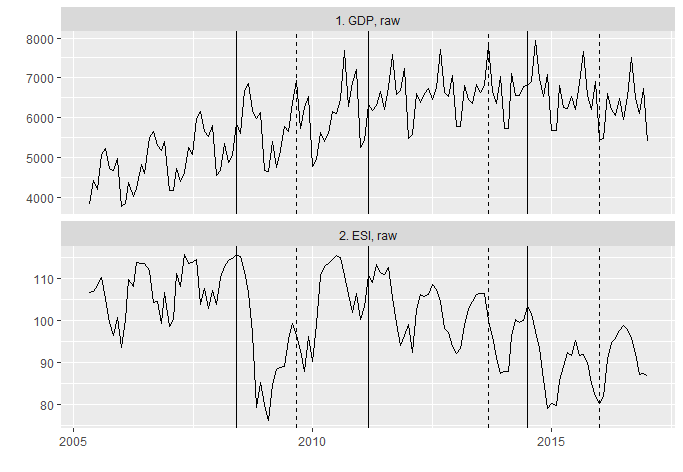
\includegraphics[width=400pt]{raw.png}
		\caption{Исходные ряды ВВП и ИЭН}
	\end{figure} 
	
	
	\section{Исследование метода выделения циклов на основе фильтра Ходрика – Прескотта}
	Рассматривались ряды, предварительно сезонно скорректированны процедурой X13-ARIMA-SEATS с помощью пакета Python \textbf{statsmodels} \cite{statsmodels}. Используя вышеописанную процедуру двойной фильтрации, получены “гладкие” ряды (обозначены smoothed). Они представлены на рис. \ref{fig:hp-gdp} и рис. \ref{fig:hp-esi}. На всех графиках вертиальными чертами указываны поворотные точки ВВП, полученные экспертными оценками (сплошная соответствует пику, штрихованная – дну).
	
	\begin{figure}
		\label{fig:hp-gdp}
		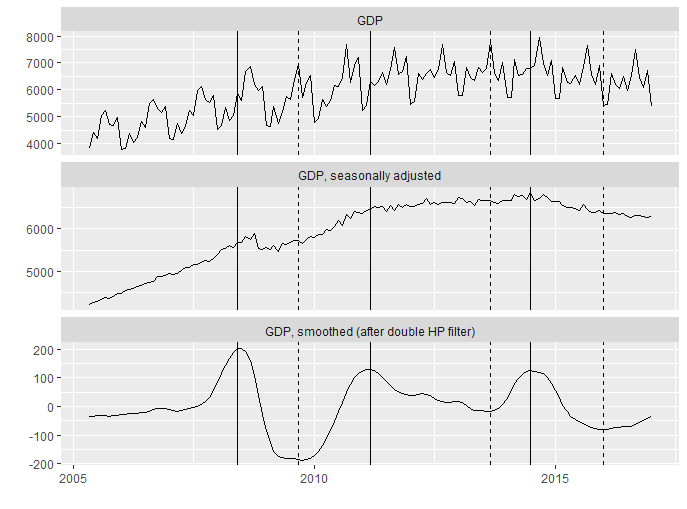
\includegraphics[width=\linewidth]{gdp_base-sa-hp.png}
		\caption{ВВП, исходная серия (первый ряд), после сезонной корректировки (второй ряд), и после удаления тренда двойным применением фильтра Ходрика – Прескотта (нижний ряд).}
	\end{figure}
	
	\begin{figure}
		\label{fig:hp-esi}
		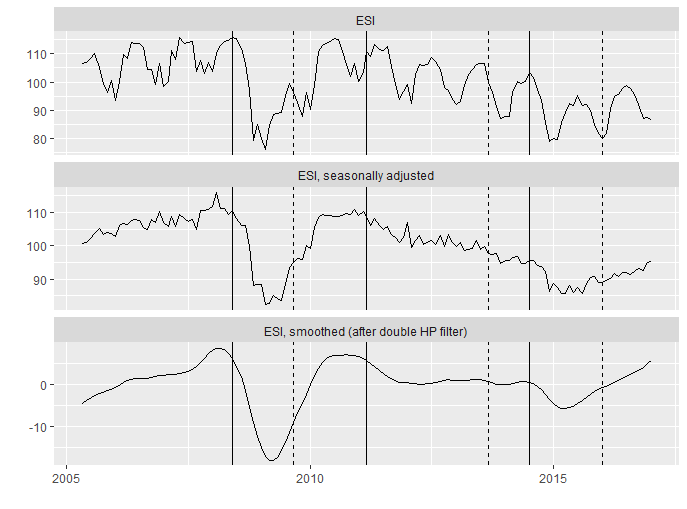
\includegraphics[width=\linewidth]{esi_base-sa-hp.png}
		\caption{ИЭН, исходная серия (первый ряд), после сезонной корректировки (второй ряд), и после двойного применения фильтра Ходрика – Прескотта (нижний ряд).}
	\end{figure}
	
	Как видно на рис. \ref{fig:hp-ptcompare}, полученный ряд ИЭН опережает ВВП на 4-5 периодов (месяцев), что подтверждает также кросс–корреляционная функция для сглаженных рядов (см. рис. \ref{fig:ccf}). Самая сильная кросс–корреляция отмечается на этих лагах, слегка выше на четвертом. Это типичный результат для опережающих индикаторов. Также видно из рис. \ref{fig:hp-ptcompare}, что пики и локации дна в сглаженном ВВП в целом соответствуют официальным поворотным точкам. Это дает уверенность в том, что этот метод выделения циклов работает для белорусской экономики.
	
	\begin{figure}
		\label{fig:ccf}
		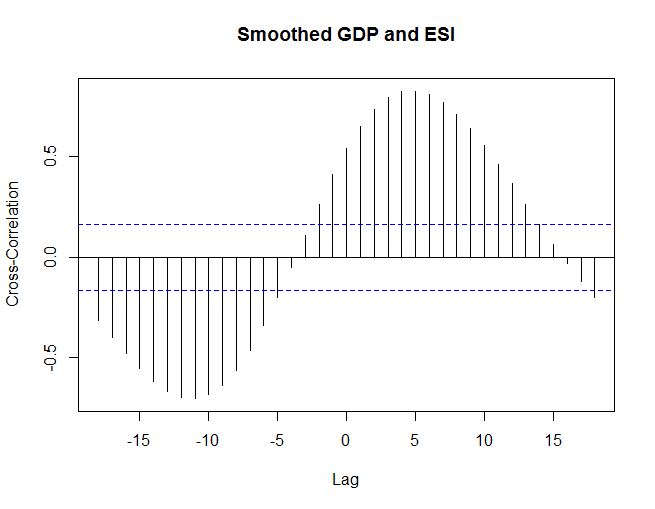
\includegraphics[width=\linewidth]{gdp_esi_crosscorr.png}
		\caption{Кросс–корреляция ВВП и ИЭН. Виден максимум на лагах 4-5.}
	\end{figure}	
	
	\begin{figure}
		\label{fig:hp-ptcompare}
		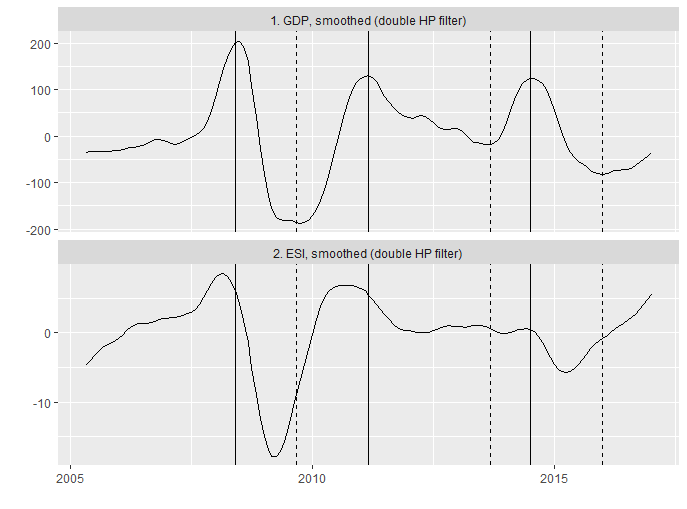
\includegraphics[width=\linewidth]{both_sm_tp.png}
		\caption{Сравнение поворотных точек сглаженных ВВП и ИЭН.}
	\end{figure}
	
	\section{Исследование метода Хамильтона и его сравнительный анализ с методом на основе фильтра Ходрика – Прескотта}
	В работе также рассматривались и ряды, скорректированные по методу Хамильтона. Эта корректировка проводилась двумя способами: без предварительной сезонной корректировки и с сезонной корректировкой с помощью X13-ARIMA-SEATS \cite{seasonalManual}. Частичная регрессия (subset regression) вида $ARp(12,13,14,15)$, которая требуется для корректировки по Хамильтону, проведена с помощью пакетов R \textbf{MSwM} и Python \textbf{statsmodels} \cite{statsmodels}. Для определения поворотрых точек ряды сглаживаются высокочастотным фильтром Ходрика – Прескотта ($\lambda=13.93$). Результаты преведены на рис. \ref{fig:gdp_compare}, включая варианты с предварительной сезонной корректировкой.  После корректировки по Хамильтону получаются похожие поворотные точки, но они могут отличатся на пару месяцев в разных направлениях. Ряды, скорректированные сезонно и по Хамильтону, имеют более схожие поворотные точки, с отклонениями в пару месяцев. Нужно также отметить, что первые $h=12$ наблюдений в рядах, скорректированных по Хамильтону, необходимо исключать из моделирования.
	
	
	\begin{figure}
		\label{fig:gdp_compare}
		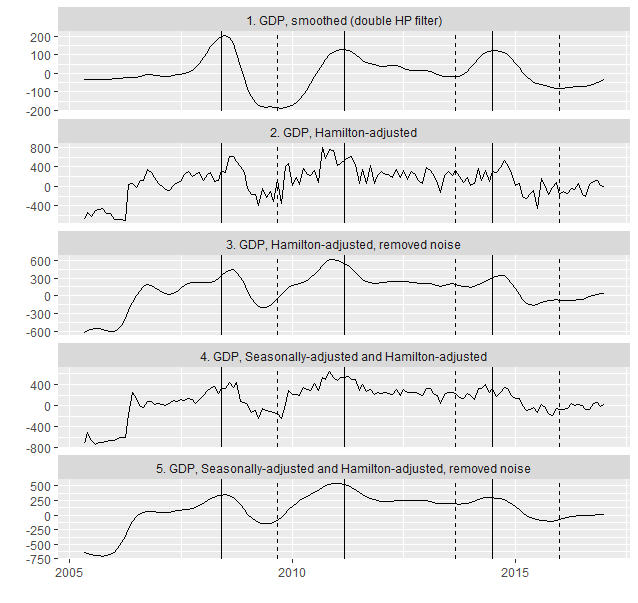
\includegraphics[width=0.8\linewidth]{gdp_compare.png}
		\caption{Сравнение результатов методов выделения цикла на основании 
			методов Ходрика – Прескотта и Хамильтона}	
	\end{figure}
	
	В конце главы приведена табл. \ref{tbl:tpoints} сравнения поворотных точек GDP, получены вышеописанными методами (а так же моделями MS-ARX, которые описаны в следующей части). Как видно, разные методы обработки временных рядов приводят к похожим, но не одинаковым оценкам времени поворотных точек (нагляднее всего это видно на рис. \ref{fig:gdp_compare}). Предлагается проводить сезонную корректировку до применения метода Хамильтона для получения значения поворотных точек, максимально близких к официальным \cite{makarevich_hse_paper,makarevich_bsu_conf_2017}.
	
	На основании результатов анализа приведенных в рис. \ref{fig:hp-gdp}–\ref{fig:gdp_compare}, а также в табл. \ref{tbl:tpoints}, можно подтвердить применимость алгоритма Хамильтона для выделения циклов. Поворотные точки циклов ВВП и ИЭН, полученные на основе данного алгоритма, либо совпадают с экспертными оценками, либо отличаются на 1–2 месяца в сторону опережения. Главное несоответствие  возникает в периоде 2011–2013 гг., который характеризуется высокой неопределенностью экономической конъюнктуры.
	
	
	\section{Анализ циклических изменений и оценка поворотных точек экономических циклов на основе модели MS-AR}
	
	Для временного ряда, скорректированного по Хамильтону, было построено несколько моделей $MS(L)-AR(p)-X(esi_{-k})$ с параметрами $L \in \{2,3\}$, $p \in \overline{0,3}$, $k \in \overline{-1,6}$. Для сравнения моделей использовались критерии:
	
	- Значимость коэфициентов модели во всех режимах
	
	- Критерий Акаике AIC
	
	- Пороговое значение частоты переключения режимов (от 2 до 10 переключений). Это условие – проверка на адекватность режимов.
	
	В результате была выбрана модель для ${GDP}$ со спецификацией $MS(2)-AR(0)-X({ESI}_{-4})$. Она соответствует уравнениями \ref{eq:msvarx} и \ref{eq:msvarx_m}).
	
	{

		\begin{equation}
			\label{eq:msvarx}
			\begin{cases}
				{GDP}_{t} = 
					\underset{-7.827}{-0.2042} 
					- \underset{-3.672}{0.3326} {ESI}_{t-4}
					+ \nu_{t} , \space \nu_{t} \sim N(0, 0.0429)
					, \quad l=0 \\
				{GDP}_{t} = 
					\underset{17.33}{0.4447}
					- \underset{-4.076}{0.2337} {ESI}_{t-4}
					+ \nu_{t} , \space \nu_{t} \sim N(0, 0.0241)
					, \quad l=1
			\end{cases}			
		\end{equation}
		\begin{equation}
			\label{eq:msvarx_m}
			M = 
				\begin{bmatrix}
				0.9787 & 0.0213 \\
				0.0313 & 0.9687
				\end{bmatrix}
			, \quad m_{i,j} = p[i \rightarrow j]
		\end{equation}
	
	}
	
	где $m_{i,i} = p[i \rightarrow i]$ – вероятность остаться в режиме $i$. Все коэффициенты оказались значимыми на уровне $0.05$. Графики с режимами представлены на рис. \ref{fig:hp-fitcompare}, его остатки описаны на рис. \ref{fig:hp-residcomp}.
	
	{
		\begin{figure}
			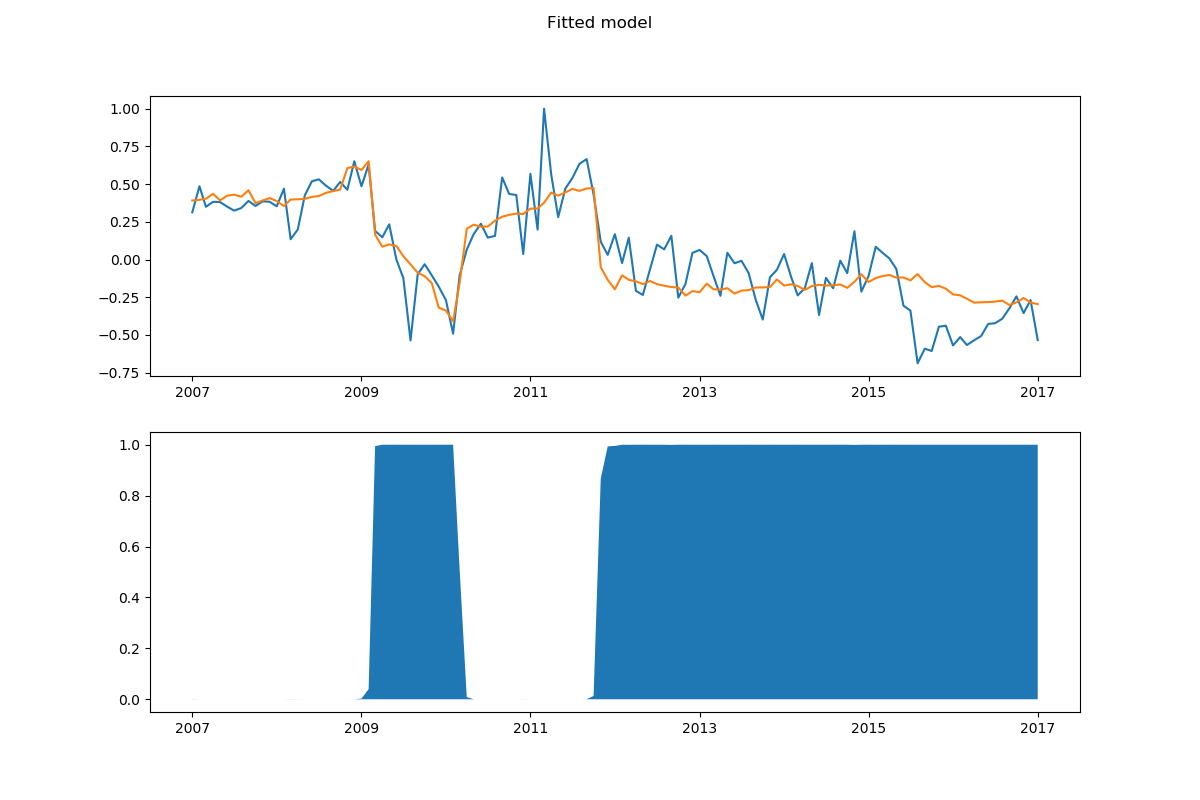
\includegraphics[width=\linewidth]{m0_fit.png}
			\caption{Предсказание модели MS(2)-ARX для ВВП по Хамильтону.}
			\label{fig:hp-fitcompare}
		\end{figure}
		\begin{figure}
			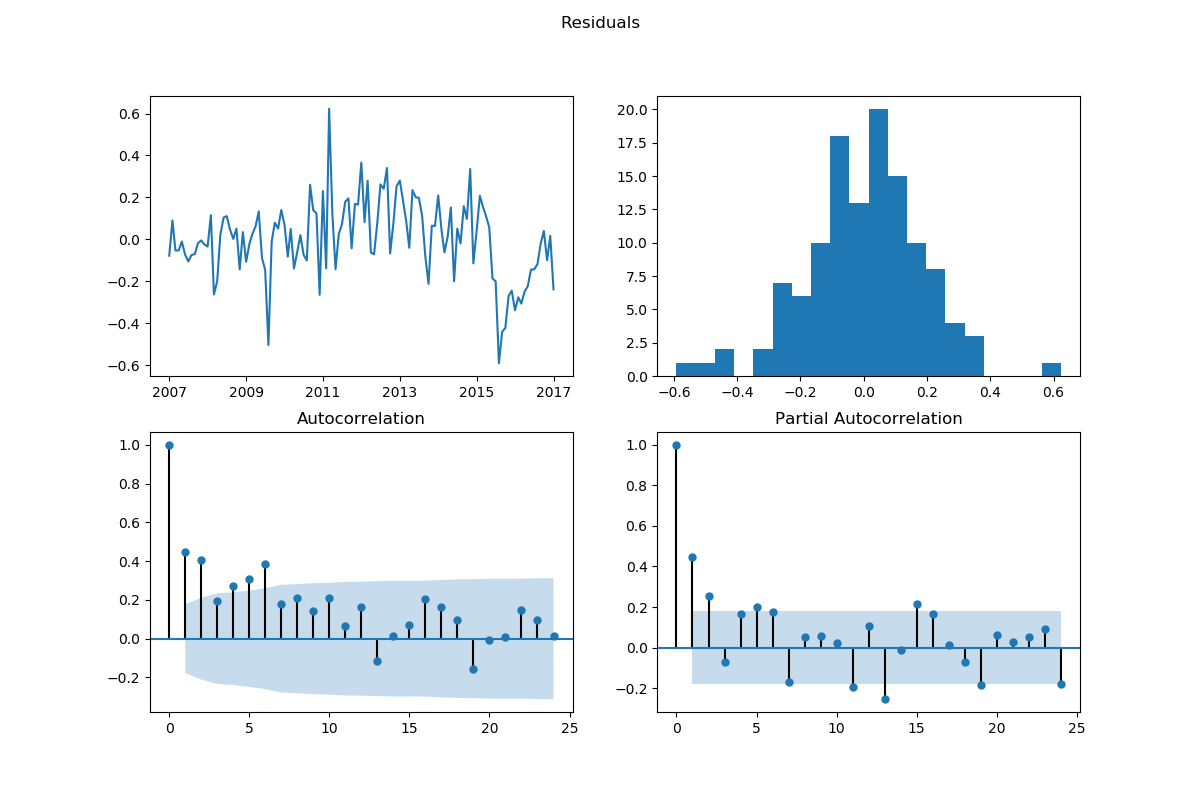
\includegraphics[width=\linewidth]{m0_resid.png}
			\caption{Анализ остатков модели для ВВП по Хамильтону.}
			\label{fig:hp-residcomp}
		\end{figure}
	}
	
	
	Аналоничным методом была построена модель для годовых темпов роста ВВП и ИЭН\footnote{от обоих рядов отнята единица для центровки}. Была выбрана модель со спецификацией $MS(2)-AR(0)-X({ESI}_{-2})$. Модель для темпов ростов исходных рядов соответствует уравнениям \ref{eq:ms2varx} и \ref{eq:ms2varx_m}.
	
	Графики ВВП, модельных значений, режимов, и анализа остатков так же приведены (рис. \ref{fig:hp-fitcompare2}, \ref{fig:hp-residcompare2}).
	
	
	{
	\begin{equation}
		\label{eq:ms2varx}
		\begin{cases}
			{GDP}_{t} = 
				\underset{-2.060}{-0.007623} 
				- \underset{-3.333}{0.1432} {ESI}_{t-2}
				+ \nu_{t} , \space 
				, \quad l=0 \\
			{GDP}_{t} = 
				\underset{21.78}{0.09731}
				- \underset{-2.785}{0.1030} {ESI}_{t-2}
				, \quad l=1 \\
			\nu_{t} \sim N(0, 0.000786) , \quad l \in \{0, 1\}
		\end{cases}	
	\end{equation}
	\begin{equation}
		\label{eq:ms2varx_m}
		M = 
			\begin{bmatrix}
			0.9787 & 0.0213 \\
			0.0313 & 0.9687
			\end{bmatrix}
		, \quad m_{i,j} = p[i \rightarrow j]
	\end{equation}		
	}
		
	{
		\begin{figure}
			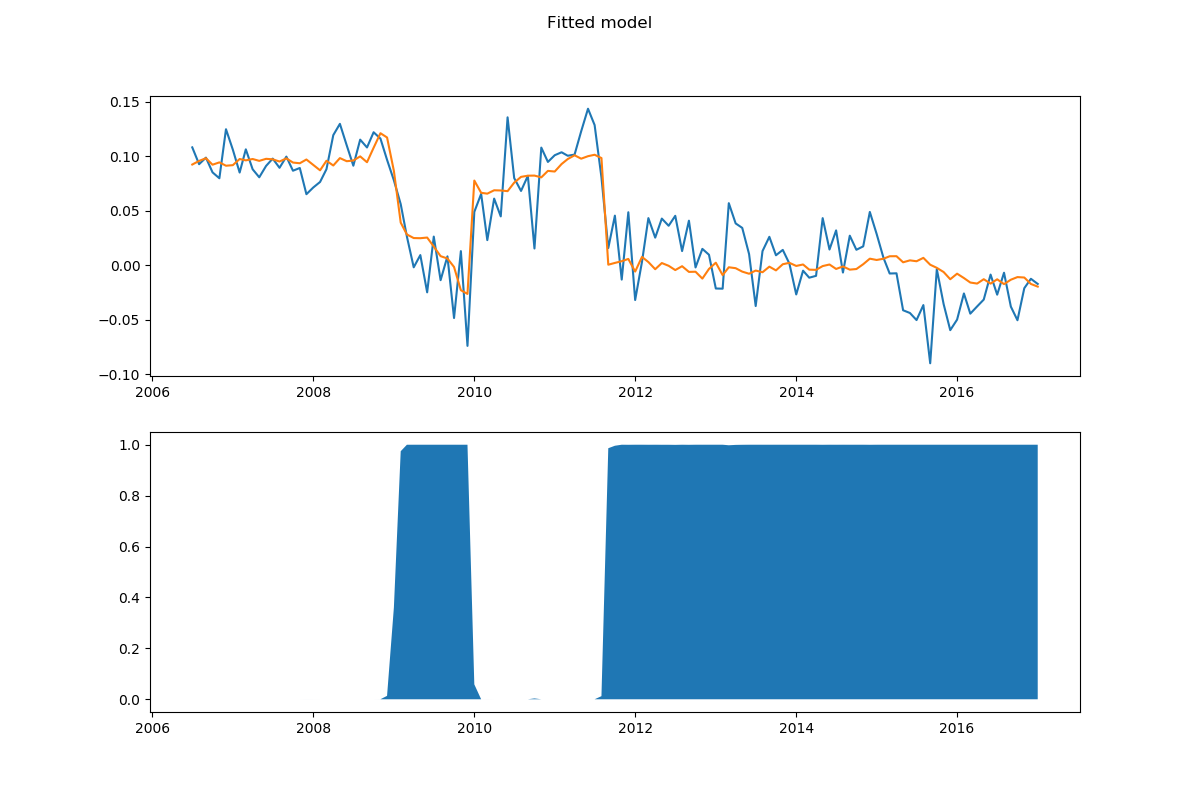
\includegraphics[width=\linewidth]{t2_fit.png}
			\caption{Предсказание модели MS(2)-ARX для темпов роста ВВП.}
			\label{fig:hp-fitcompare2}
		\end{figure}
		\begin{figure}
			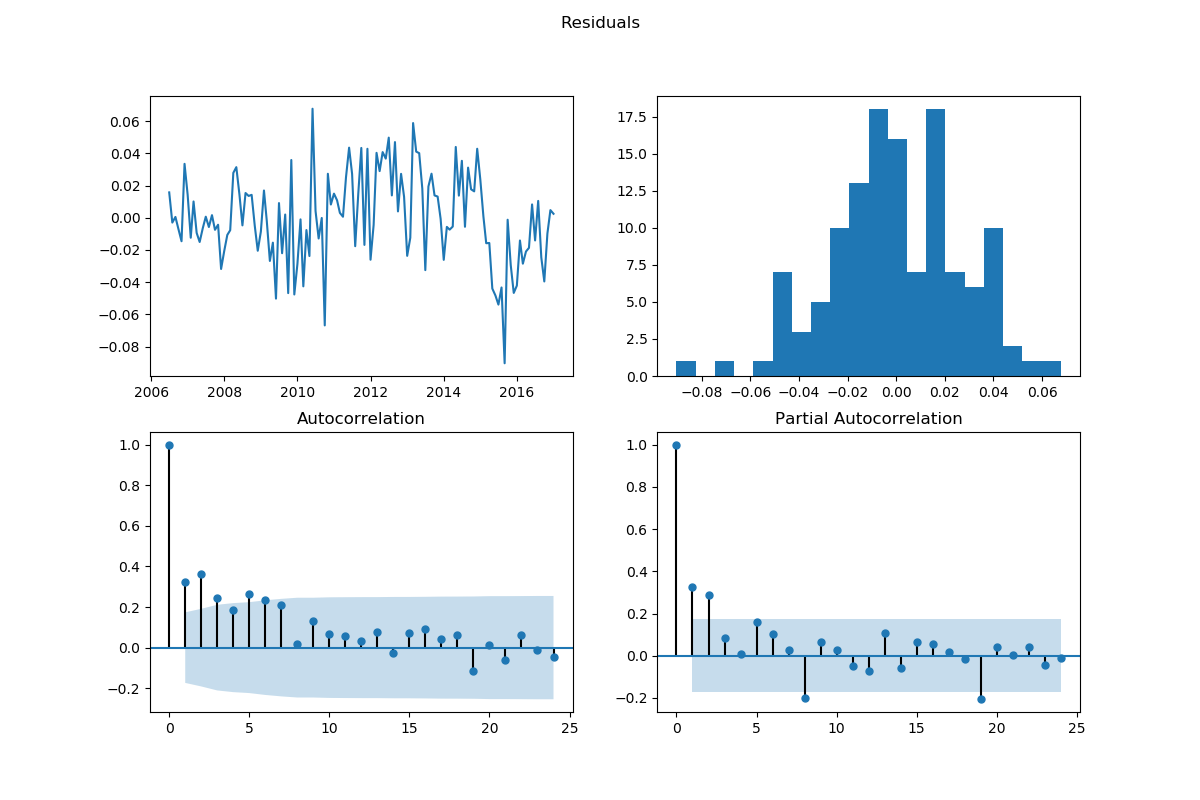
\includegraphics[width=\linewidth]{t2_resid.png}
			\caption{Анализ остатков для модели темпов роста ВВП.}
			\label{fig:hp-residcompare2}
		\end{figure}
	}
	
	\section{Сравнительный анализ и экономическая интерпретация поворотных точек на основе различных методов }
	
	
	В табл. \ref{tbl:tpoints} приведены оценки поворотных точек разными методами. В качестве «истинных» значений рассматриваются экспертные оценки. Как видно, лучше всего совпадают точки, полученные в ходе двойной фильтрации (конкретно, для одной точки предсказание опаздывает на 1 месяц). Однако, точки полученные по Хамильтону (после сглаживания) отличаются не более чем на 2 месяца, причем всегда с опережением.
	
	На основании приведенных в графиках и таблице результатов можно подтвердить применимость алгоритма Хамильтона для выделения циклов. Поворотные точки циклов ВВП и ИЭН, полученные на основе данного алгоритма, либо совпадают с экспертными оценками, либо отличаются на 1–2 месяца в сторону опережения.
	
	Точки переключения режимов моделей–подклассов MS-VARX для различных рядов сильнее отличаются от истинных поворотных точек. В сравнении с другими моделями, MS-ARX для рядов, скорректированных по Хамильтону более точно предсказала первые две точки, а также третий пик, но «пропустила» период 2011–2013 года. Есть предположение, что моделирование с помощью MS-VARX позволит этот период описать точнее. В заключающей части этой работы производится разработка библиотеки, упрощающая создание такой модели.
	
	
	
	\begin{table}[]
		\label{tbl:tpoints}
		\caption{Сравнение поворотных точек, полученные разными методами.}		
		\begin{tabular}{l|c|c|c|c}
			\textbf{Метод}                                                                   & \multicolumn{1}{l}{\textbf{(пик 1)}} & \multicolumn{1}{l}{\textbf{(дно 1)}} & \multicolumn{1}{l}{\textbf{(пик 2)}} & \multicolumn{1}{l}{\textbf{(дно 2)}} \\
			\hline
			Экспертные оценки                                                                & 2008.06                              & 2009.09                              & 2011.03                              & 2013.09                              \\
			Двойной HP filter                                                                & 2008.06                              & 2009.10                              & 2011.03                              & 2013.09                              \\
			X13 + Hamilton (сглаж.)                                                          & 2008.06                              & 2009.07                              & 2011.01                              & 2013.09                              \\
			\begin{tabular}[c]{@{}l@{}}MS-VAR для \\ индикаторов доверия\end{tabular}        & 2008.10                              & 2009.02                              & 2011.03                              & 2012.06                              \\
			\begin{tabular}[c]{@{}l@{}}MS-ARX для темпов\\ роста ВВП (экзогенная – ИЭН)\end{tabular} & 2009.01                              & 2010.01                              & 2011.09                              & -                              \\
			\begin{tabular}[c]{@{}l@{}}MS-ARX для Hamilton\\ ВВП (экзогенная – ИЭН)\end{tabular}     & 2009.01                              & 2009.11                              & 2011.08                                    & -                                   
		\end{tabular}
		
		\begin{tabular}{l|c|c|c}
			\textbf{Метод}                                                                   & \multicolumn{1}{l}{\textbf{(пик 3)}} & \multicolumn{1}{l}{\textbf{(дно 3)}} & \multicolumn{1}{l}{\textbf{Замечания}} \\
			\hline
			Экспертные оценки                                                                & 2014.07                              & 2016.01                              & Официальные оценки                            \\
			Двойной HP filter                                                                & 2014.07                              & 2016.01                              & Методика совпадает с офиц.                                       \\
			X13 + Hamilton (сглаж.)                                                          & 2014.06                              & 2015.11                              &  \\
			\begin{tabular}[c]{@{}l@{}}MS-VAR для \\ индикаторов доверия\end{tabular}        & 2014.11                              & -                                    & см. \cite{coursework_babakhin}                  \\
			\begin{tabular}[c]{@{}l@{}}MS-ARX для темпов\\ роста ВВП (экз. ИЭН)\end{tabular} & -                              & -                                    &                      \\
			\begin{tabular}[c]{@{}l@{}}MS-ARX для Hamilton\\ ВВП (экз. ИЭН)\end{tabular}     & -                              & -                                    & 
		\end{tabular}
		
	\end{table}
	
	
	\chapter{Прогностическая способность моделей}
	
	При анализе экономических показателей, часто ставится цель прогнозирования будущего состояния временных рядов. На основании этих прогнозов выбираются стратегии дальнейших действий. Исторически, для достижения этой цели использовались авторегрессионные модели; модели MS-VARX являются расширением этого класса, поэтому возникает вопрос об их прогнозной способности в сравнении с ``обычными'' методами.
	
	\section{Задача валидации модели}
	
	Для оценивания прогнозной способности моделей линейной регрессии часто используется процедура, которая называется ``кросс–валидация'', в которой случайная часть тренировочного набора выбирается в качестве тестовой выборки для оценивания поведения модели на ``новых'' данных. Однако при применении для моделирования временных рядов эта процедура имеет серъезные недостатки. Во–первых, если выбрасывать данные из ``середины'' временного ряда, то становится невозможным предсказание последующих наблюдений. Во–вторых, из–за серийной корреляции оценка ошибки предсказания будет значительно ниже чем действительное значение. Так же возникает проблема с недостатком данных, если есть только одна реализация временного ряда не очень большой длины, и характеристики ряда могут меняться со временем.
	
	Воизбежание этих проблем используется процедура ``скользящей валидации''. Алгоритм состоит в следующим (наглядный пример ниже):
	\begin{enumerate}
		\item Выбор длины валидации $L$ для временного ряда  $y_t$ длиной $T$.
		\item Для значений $l \in \{L, L-1, ..., 1\}$:
		\begin{enumerate}
			\item Оценивается модель на данных $y_1..y_{T-l}$
			\item Вычисляется ошибка прогноза на один шаг вперед: 
			$\hat{\varepsilon}_{T-l+1} = y_{T-l+1} - \hat{y}_{T-l+1}$
		\end{enumerate}
		\item Считается оценка метрики (часто – среднеквадратичное или среднее абсолютное отклонение) по $\hat{\varepsilon}_{T-L+1} ... \hat{\varepsilon}_{T}$, которая в дальнейшем используется для будущих прогнозов данного ряда.
	\end{enumerate}
	
	\begin{figure}
		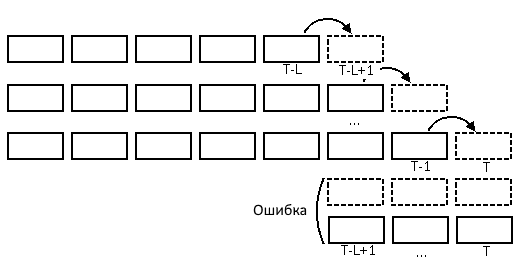
\includegraphics{RollingValidation.png}
		\caption{Принцип скользящей валидации.}
		\label{fig:rolling_validation}
	\end{figure}
	
	Существуют и другие методологии (хороший обзор проведен в \cite{hyndCV}), но из–за небольшой длины исходных временных рядов, скользящая валидация считается самой точной.
	
	
	\section{Сравнение точности прогнозов моделей для ВВП}
	
	Вышеописанный подход ``скользящей валидации'' был использован для оценки точности прогноза для описанных моделей MS-ARX для годовых темпов роста ВВП (GRGDP) и для ВВП, скорректированого по Хамильтону (HamGDP). В качестве ``обычных'' методов для обоих рядов рассматривались модели модели $SARIMAX$ с автоматически подобранными порядками (алгоритм выбора описан в \cite{hynd_autoarima} и имплементирован в пакете Python \textbf{pyramid\_arima} \cite{pyramid_arima}). В таблице \ref{tbl:errors} указаны среднеабсолютые (MAE) и среднеквадратичные (RMSE) ошибки прогнозов моделей для ВВП, скорректированные по Хамильтону, и для годовых темпов роста ВВП. Ниже представлены графики прогнозов моделей.
	
	\begin{figure}
		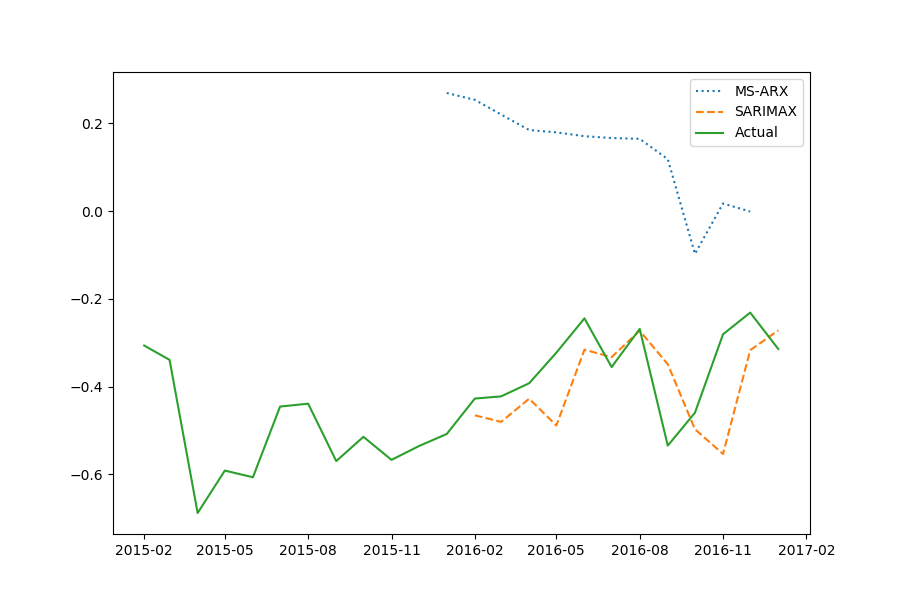
\includegraphics[width=400pt]{compare_ham.png}
		\caption{Сравнение скользящих прогнозов по Хамильтону.}
		\label{fig:rollcompare-ham}
	\end{figure}
	
	\begin{figure}
		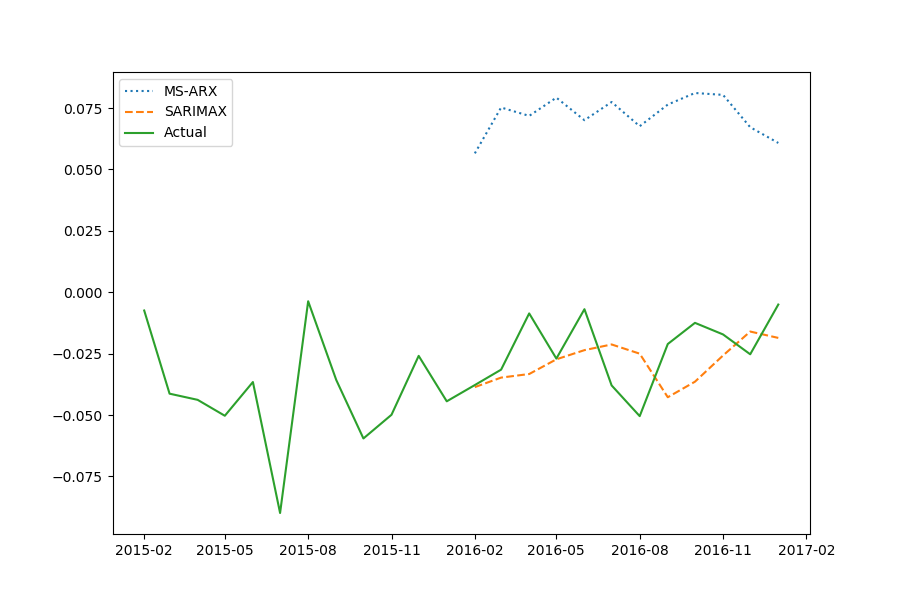
\includegraphics[width=400pt]{compare_gr.png}
		\caption{Сравнение скользящих прогнозов для темпов роста ВВП.}
		\label{fig:rollcompare-tr}
	\end{figure}
	
	\begin{table}[]
		\centering
		\caption{Сравнение ошибок прогонзов}
		\label{tbl:errors}
		\begin{tabular}{llll}
			& Метрика & MS-ARX & SARIMAX \\
			\multirow{2}{*}{ВВП по Хамильтону} & MAE    & 0.5646 & 0.0850  \\
			& RMSE   & 0.6019 & 0.1150  \\
			\multirow{2}{*}{Годовые темпы роста}       & MAE    & 0.0988 & 0.0137  \\
			& RMSE   & 0.1005 & 0.0164 
		\end{tabular}
	\end{table}
	
	
	Как видно, модели $MS(2)-AR(0)X$ сильно уступают подобраным моделям $SARIMAX$. Можно сделать вывод, что модели переключения среднего значения не годятся для предсказывания ВВП, а только для классификации прошлых периодов (циклов) и оценивания поворотных точек.
	
	
	\chapter{Разработка библиотеки Time Series for Data Science}
	
	Одно из направлений дальнейших исследований – векторные модели переключения состояния (MS-VARX) для отдельных секторов экономики РБ. Для оценивания параметров такой модели уже разработан EM–алгоритм \cite{malNovopMSVARX}, но он не воплощен ни в одном пакете для языков R и Python. Другое направление – оценивание параметров при известных значениях поворотных точек, для чего также не существует пакета.
	
	Реализация алгоритмов оценивания требует больших усилий, включая работы над формализацией входных данных, проверкой предположений и выводом результатов. Для проверки корректности работы этих алгоритмов, необходимо иметь возможность сравнивать их результаты с результатами других моделей существующих пакетов. Наконец, для упрощения сравнения результатов разных моделей удобно представлять их в одинаковом формате.
	
	По этим причинам и на основания опыта работы в дисциплине «data science», автором была разработана библиотека «Time Series for Data Science» (коротко – \textbf{ts4ds}) на языке программирования Python. 
	
	\section{Краткое описание и основные задачи}
	
	\textbf{Time Series for Data Science} (сокращенно – \textbf{ts4ds}, на русском – «Временные Ряды для Анализа Данных») – пакет для языка программирования Python, написанный автором во время практики в компании «ЭПАМ Системз» (EPAM Systems). Он включает в себя средства для анализа и прогнозирования временных рядов, а также средства для разработки новых моделей. С точки зрения программного кода, он содержит базовые классы, разработанные модели, утилиты и программные тесты.
	
	При проектировании и написании пакета \textbf{ts4ds}, были поставлены следующие задачи:
	\begin{itemize}
		\item использовать методы статистического и машинного обучения для построения эконометрических моделей временных рядов;
		\item разработать обобщенное представление модели временных рядов, с целью автоматизации процессов ее построения и применения;
		\item реализовать в библиотеке процедуры построения, применения некоторых основных семейств моделей
		\item реализовать процедуры автоматизации работы с моделями (например, поиск гипер–параметров);
		\item разработать утилиты для облегчения создания новых моделей;
		\item провести тестирование компонент библиотеки (в программном и в статистическом смысле).
	\end{itemize}
	
	\section{Принципы разработки библиотеки}
	
	Для выполнения поставленных задач был необходим фундаментальный подход к проектированию и разработке библиотеки. В качестве основы брались идеи как из эконометрики, так и из дисциплины машинного обучения. Следует пояснить некоторые термины, взятые из этих дисциплин:
	
	\textbf{Модель} – объект, описывающий (и, возможно, предсказывающий) поведение временных рядов. Математически, модель представляется параметризованными уравнениями, описывающи отношения между переменными. Эти переменные можно условно разбить на \textbf{эндогенные} (объясняемые моделью) и \textbf{экзогенные} (не объясняемые, а взятые извне и неизменяемые внутри модели).
	
	\textbf{Предиктивные модели} позволяют строить прогнозы значений временных рядов. Примерами являются авторегрессионные модели, экспоненциальное сглаживание, и рекуррентные нейросети.
	
	\textbf{Преобразования} временных рядов изменяют значения временного ряда по определенному принципу, получая при этом новый ряд. Примерами являются взятие разностей, сезонная корректировка, и методы декорреляции. (При разработке библиотеки оказалось, что преобразования удобно рассматривать как вид моделей.)
	
	\textbf{Параметры} модели – обозначения их коэффициентов, а также значения этих коэффициентов. Иногда отдельно выделяют гиперпараметры, которые влияют на саму форму модели, но в пакете \textbf{ts4ds} такое отличие не делается.
	
	\textbf{Эстиматор} (от англ. estimator) – алгоритм, который ищет оптимальную (по какому–то критерию) модель. Обычно этот поиск происходит в пространстве параметров, т.е. это алгоритмы оценивания параметров.
	
	Удобно рассматривать множество всевозможных моделей как функциональное пространство зависимостей между переменными. Конкретные классы моделей выделяют подмножества моделей, «точки» в предложенном функциональном пространстве, которые характеризуются определенной параметризацией. Например: множество линейных авторегрессионных моделей скалярной величины $AR(p)$ включают в себя подмножество авторегрессии второго порядка $AR(2)$, которое в свою очередь включает конкретную модель $AR(2)$ с коэффициентами $[-0.61, 0.22]$. В такой постановке эстиматоры можно рассматривать как алогритмы нахождения оптимальной точки (комбинации параметров) в некотором подпространстве.
	
	\section{Особенности имплементации}
	
	В библиотеке \textbf{ts4ds} каждой из вышеописанных частей соответствует отдельный класс объектов. В рамках пакета данные представляются в виде многомерного массива (numpy.ndarray) либо индексированной таблицей (pandas.Series/DataFrame) – что является стандартом представления во всех научных библиотеках Python. Все модели – наследники класса Model и дополнительных классов (Predictor, Transformer) с соответствующими параметрами, унаследованные от Parameters, и стандартными по интерфейсу процедурами. Эстиматоры (наследованные от Estimator) воплощают вышеописанные алгоритмы и возвращают объекты моделей вместе с параметрами.
	
	Стоит отметить, что такая организация несколько отличается от большинства традиционных библиотек. Во многих библиотеках (например, \textbf{scikit-learn}, \textbf{statsmodels}\cite{statsmodels}, и многих библиотеках языка R) процедуры оценивания параметров и процедуры выдачи предсказаний совмещены в один объект. Часто в этой структуре заодно хранят и данные. Этот подход обоснован традиционным применением: эконометрическая модель строится на одной  реализации процесса и анализируется вручную. Однако, как показывает практика, для многих промышленных применений такой традиционный подход значительно ограничивает потенциал автоматизации. 
	
	Главные недостатки традиционной организации (т.е. такой, как в \textbf{statsmodels}):
	
	\begin{itemize}
		\item неудобно сохранять модели компактно, так как нет явного понятия «минимальных данных для воспроизведения»;
		\item эстиматоры, которые оценивают одинакове модели (например, МНК и LASSO), должны заново воплотить процедуру предсказания; тем более, могут быть эквивалентные репрезентации, которые усложняют сравнение вычисленных параметров для одинаковых моделей;
		\item модели «привязаны» к данным, что делает невозможным их применение даже к данным относительно среднего размера, не говоря уже о «больших данных»;
		\item многие алгоритмы машинного обучения, особенно нейросети, построены с использованием отдельных структур модели, метода оценивания и данных.
	\end{itemize}
	
	Подход привязывания данных легко «включить» в \textbf{ts4ds}: для сохранения этой функциональности, а также и краткости записи, существует возможность «привязать» данные к модели через обертку BoundModel. Кроме компактной дополнительной нотации в программном коде, особых недостатков у подхода «разделения ролей» нет.
	
	\section{Результаты разработки}
	
	Базовые классы в библиотеке \textbf{ts4ds} – Parameters (параметры), Model (модель), Estimator (эстиматор/алгоритм оценивания). Эти классы описывают стандартные интерфейсы для наследующих классов и, совместно с функциями в отделе «devtools», освобождают от рутинной работы (например, проверки входных данных). На их основе воплощены некоторые популярные модели (и эстиматоры для них). Они служат как готовыми продуктами, которые можно использовать в работе аналитика или эконометриста, так и примерами имплементации для разработчиков собственных моделей. Все модели и эстиматоры, а также и часть утилит, автоматически проверяются программными тестами на правильность реализации конвенций интерфейса и на сходство результатов выполнения на тестовых данных.
	
	%\subsection{Базовые классы}
	
	Объект параметров (Parameters) – набор пар ключ–значение, соответствующие именованным параметрам какой–нибудь модели, функции проверки допустимости параметров и другие вспомогательные функции.
	
	Объект модели (Model) включает в себе значение параметров и функции предсказаний (predict).
	
	Объект эстиматора (Estimator) включает в себе настройки/параметры алгоритма оценивания и реализацию этого алгоритма (fit), которая принимает набор данных и возвращает объект модели с соответствующими параметрами.
	
	%\subsection{Преобразования}
	
	Преобразования временных рядов наследованы от классов Model и Transformer. В общем случае, у преобразования существует обратное преобразование, и его форма зависит от преобразуемых данных. Поэтому удобно рассматривать преобразование как вид модели, с соответсвующими параметрами (необходимая информация для прямого и обратного преобразования) и эстиматором, который получает эти параметры. Этот подход позволяет реализовывать обратимые преобразования.
	
	В пакете на текущий момент включены следующие преобразования:
	\begin{itemize}
		\item обычные и сезонные разности, для скаляров и векторов, и обратные процедуры интегрирования;
		\item цепные трансформации, т.е. композиция преобразований.
	\end{itemize}
	
	Планируется добавить следующие преобразования:
	\begin{itemize}
		\item применение скалярных и векторных функций к каждому периоду (и, при возможности, их обратные функции);
		\item наивная сезонная декомпозиция;
		\item сезонная корректировка по процедурам X13-ARIMA-SEATS, TRAMO-SEATS;
		\item процедура выделения тренда по Хамильтону.
	\end{itemize}
	
	Ниже приведен пример работы с преобразованием взятия разности:
	
	\begin{lstlisting}[language=Python]
	from ts4ds.models.transforms.difference import Diff
	from ts4ds.models.transforms.chain import Chain_Estimator as Chain
	from ts4ds.datasets.stata_data import get_air2
	import matplotlib.pyplot as plt
	import statsmodels.api as sm
	plot_acf = sm.graphics.tsa.plot_acf
	
	y = get_air2()['lnair'] # aircraft passengers dataset
	
	# fit and transform
	dt1, y1 = Diff().fit_transform(y)
	dt12, y12 = Diff(S=12).fit_transform(y)
	dt_, y_ = Chain(Diff(), Diff(S=12)).fit_transform(y)
	
	# plotting
	fig, axs = plt.subplots(4, sharex=True)
	axs[0].plot(y)
	axs[1].plot(y1)
	axs[2].plot(y12)
	axs[3].plot(y_)
	plt.show()
	
	# Plot final ACF
	plot_acf(y_[13:], title="Final autocorrelation")
	plt.show()
	\end{lstlisting}
	
	\begin{figure}
		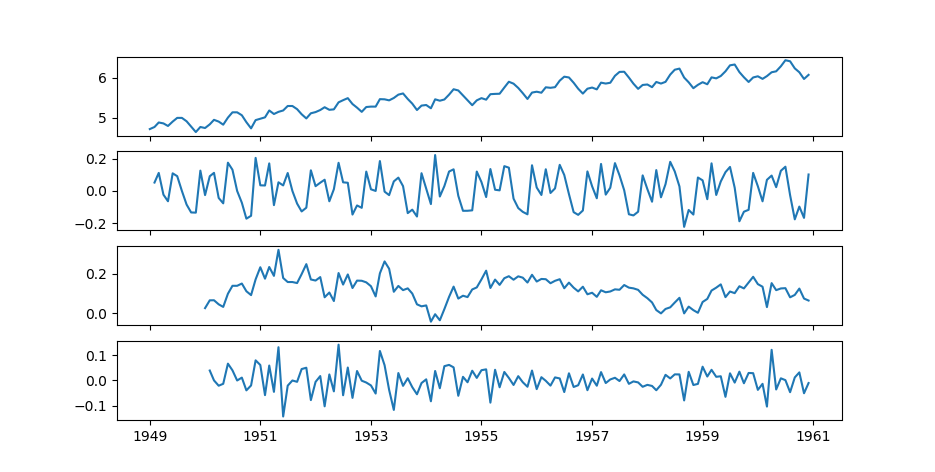
\includegraphics[width=460pt]{DiffExample.png}
		\caption{График результата выполнения (после различных трансформаций).}
		\label{fig:ts4ds-diffexample}
	\end{figure}
	\begin{figure}
		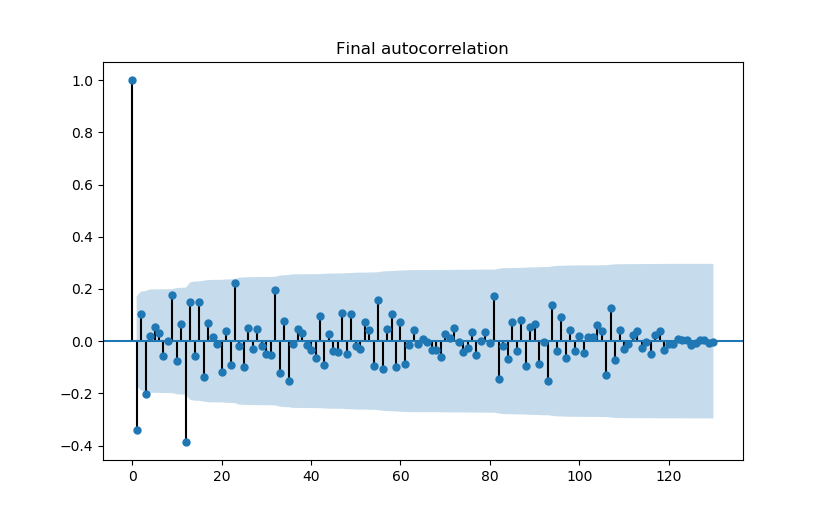
\includegraphics[width=460pt]{DiffACF.png}
		\caption{График результата выполнения (АКФ после сезонных и первых разностей).}
		\label{fig:ts4ds-diffacf}
	\end{figure}
	
	%\subsection{Предсказательные модели}
	
	В пакете \textbf{ts4ds} реализованы следующие предсказательные модели и эстиматоры для них:
	\begin{itemize}
		\item линейная регрессия;
		\item общий вид авторегрессионных моделей;
		\item модели линейной авторегрессии ARX, VARX;
		\item общая модель дискретного пространства состояний (statespace models);
		\item модели ARIMAX, SARIMAX.
		\item модели с независимыми и Марковскими переключениями состояний (семейства IS-VARX, MS-VARX).
	\end{itemize}
	
	Так же реализованы две процедуры автоматического подбора порядков для SARIMAX, так называемое «auto\_arima»\cite{pyramid_arima}. Пример реализации и использования модели SARIMAX описан ниже.
	
	Планируется добавить следующие модели и эстиматоры:
	\begin{itemize}
		\item модели переключения состояний (RS-models), включая MS-VARX;
		\item модели ARCH, GARCH;
		\item адаптеры для рекуррентных и сверточных нейросетей;
		\item адаптер для алгоритмов машинного обучения, изначально предназначенные для пространственных данных (например, SVM и регрессионные деревья).
	\end{itemize}
	
	
	\section{Пример: разработка модели SARIMAX}
	%\textbf{\Large Пример: разработка модели SARIMAX}
	
	Одна из самых распространенных моделей в анализе временных рядов – модель $SARIMAX$, которая является обобщением модели $ARMA$. Полное обозначение этой модели – $SARIMAX(p,d,q)(P,D,Q,S)$, где $S$ – порядок сезонности, $p$ и $P$ – порядки обычной и сезонной авторегрессии ($AR$), $d$ и $D$ – порядки обычной и сезонной разности ($I$), $q$ и $Q$ – порядки обычного и сезонного скользящего среднего ($MA$).
	
	Введем обозначения:
	$y_t$ – эндогенная переменная (в момент времени $t$), 
	$x_t$ – экзогенный вектор, 
	$\varepsilon_t$ – вектор ошибок, 
	$L$ – лаговый оператор, 
	$\Delta$ и $\Delta_s$ – операторы взятия обычных и сезонных разностей, 
	$\beta$ – вектор коэффициентов регрессии, 
	$\phi(\cdot)$, $\Phi(\cdot)$, $\theta(\cdot)$, $\Theta(\cdot)$ – многочлены с определенными коэффициентами $AR$ и $MA$ частей соответственно.
	
	Тогда $SARIMAX(p,d,q)(P,D,Q,S)$ можно описать в форме регрессии с остатками $SARIMA$:
	
	\begin{equation}
		\begin{cases}
			y_t = \beta^{T} x_t + u_t \\
			\Phi(L) \phi(L) \Delta_s^{Q} \Delta^{q} u_t = \Theta(L) \theta(L) \varepsilon_t \\
			\varepsilon_t \sim N(0,\sigma^{2})
		\end{cases}
	\end{equation}
	
	В случаи отсутствия экзогенных переменных, $y_t = u_t$.
	
	Для получения предсказаний в такой формулировке необходимо взять $d$ обычных и $D$ сезонных разностей, что эффективно сокращает исходный ряд на $d+SD$ периодов и усложняет задачу предсказания на эти периоды. Вместо этого, можно воспользоваться представлением в форме «пространства состояний» (statespace model) и предсказывать с помощью фильтра Калмана.
	
	Модель statespace описывается следующими уравнениями:
	\begin{equation}
		\begin{cases}
			\alpha_{t+1} = c + T \alpha_t + R \eta_t \\
			y_t = d + Z \alpha_t + \varepsilon_t \\
			\eta_{t} \sim N(0, Q) \\
			\varepsilon_t \sim N(0, H)
		\end{cases} 
	\end{equation}
	
	где $y_t$ – наблюдаемый вектор, $\alpha_t$ – латентный (скрытый) вектор состояний, $\eta_t$ и $\varepsilon_t$ – вектора ошибок в латентном и наблюдаемом векторе соответственно,
	$T$, $R$ и $Z$ – матричные параметры модели, $c$ и $d$ – вектора констант, $Q$ и $H$ – ковариационные матрицы.
	
	Представляя в таком виде $SARIMAX$, возможно делать предсказания с помощью фильтра Калмана. Этот подход используется в пакетах \textbf{statsmodels}\cite{fulton_statespace} и \textbf{ts4ds}. Реализация фильтра Калмана в \textbf{statsmodels} очень эффективная, поэтому он используется в качестве основе для предсказаний в \textbf{ts4ds}. 
	
	Ниже показан пример использования модели SARIMAX для прогнозирования на 4 периода вперед для сезонной модели, а также ряд ошибок предсказаний.
	
	\begin{lstlisting}[language=Python]
	from ts4ds.estimators.sm_wrap.sarimax import SARIMAX_Estimator
	from ts4ds.datasets.stata_data import get_air2
	import matplotlib.pyplot as plt
	import pandas as pd
	
	y = get_air2()['lnair'] # airplane passenger dataset
	oos = pd.date_range('1961-01-01', periods=4, freq='MS') # out-of-sample
	
	# fit and predict
	model = SARIMAX_Estimator(p=1, d=1, D=1, S=12).fit(y)
	y_ins = model.predict_in_sample(y)
	y_next = model.predict(oos,y)
	y_hat = pd.concat([y_ins, y_next])
	
	# plot
	fig, axs = plt.subplots(2, sharex=True)
	h1, = axs[0].plot(y, color='0.0')
	h2, = axs[0].plot(y_hat[13:], color='red', linestyle='--')
	h4, = axs[1].plot((y_hat-y)[13:], color='0.0')
	axs[0].legend(handles=[h1,h2,h3],labels=['actual','predicted'])
	plt.show()
	\end{lstlisting}
	
	\begin{figure}
		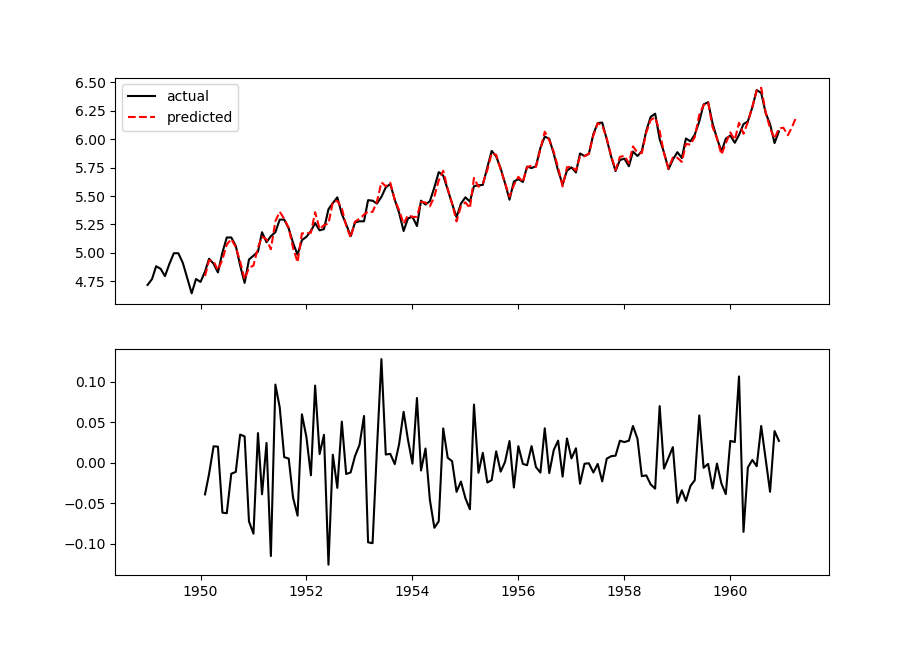
\includegraphics[width=460pt]{sarimax_example.png}
		\caption{Пример работы модели SARIMAX.}
		\label{fig:ts4ds-sarimax-example}
	\end{figure}
	
	%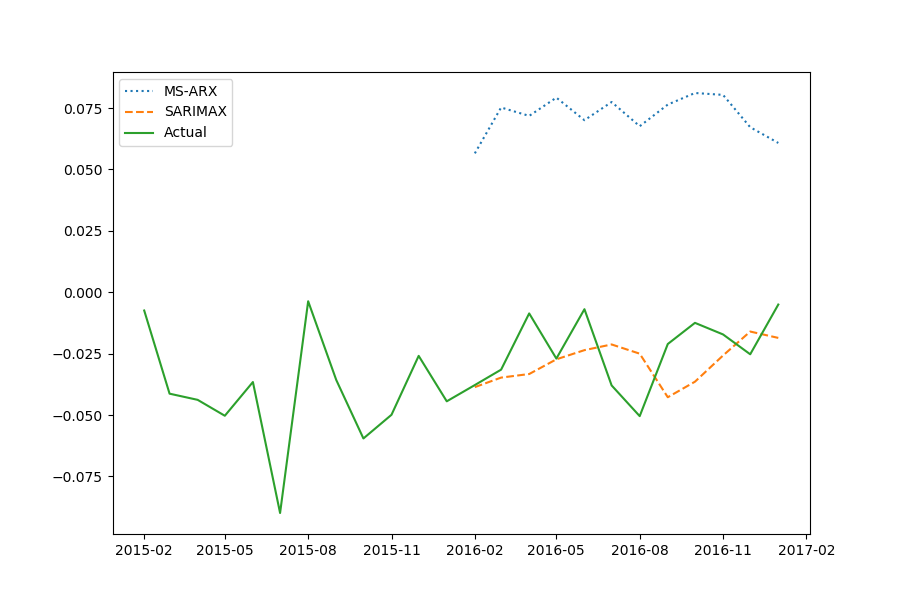
\includegraphics[width=400pt]{compare_gr.png}
	
	
\end{document}